\documentclass[12pt,letterpaper]{report}

\usepackage[latin1]{inputenc}
\usepackage{amsmath}
\usepackage{amsfonts}
\usepackage{amssymb}
\usepackage{subfig}
\usepackage{float}
\usepackage{graphicx}
\usepackage{listings}
\usepackage[left=1.00in, right=1.00in, top=1.00in, bottom=1.00in]{geometry}

\newcommand\numberthis{\addtocounter{equation}{1}\tag{\theequation}}

\title{
	Characterizing a CCD
}
\author{
	Author: Preston Went \\
	Department of Astronomy \\
	University of Washington, Seattle \\}
\date{\today}

\begin{document}

\maketitle

\section*{Introduction}

Charge-coupled devices (CCDs) are the most commonly used type of light detector in visual-range astronomy. CCDs have a high quantum efficiency, low read noise, large dynamic range, and high linearity, making them an excellent choice for sensitive measurements. However, astronomers today, as always, push the limits of the instruments available to them, necessitating a good understanding of precisely how a given CCD behaves. Here, I report on the basic characterization of a CCD.

\section*{Experimental Methods}

The experimental setup consisted of a SBIG ST-7XME CCD camera mounted facing into a dark box. I controlled the camera with CCDSoft. Characterizing a CCD requires capturing a series of bias, dark, and flat images - bias images being taken with zero exposure time and flat images being of a spatially uniform light source with a nonzero exposure time.

I took two bias images with the box closed. I then propped open the box with a pencil to let in light, and took a series of flat images with exposure times in seconds of 0.16, 0.312, 0.625, 1.25, 2.5, 5, 15, 25, 35, 45, 55, 65, 75, 85, 95, and 105. I also took two flats with the exposure time tuned such that the maximum counts in them was near 25$\,$000$\,$ADU -- about half of the saturation limit. This was to stay in the linear range.

I performed all data analysis in Anaconda 3 using instructor-provided Jupyter notebooks.

\section*{Characterization}

\subsection*{Read Noise and Gain}

The gain is our first quantity of interest. Here we will define it as the number of ADUs registered by the camera's A/D converter per electron in the pixel being read out. The essential theory of our calculation is as follows. The flat noise in ADUs is related to the gain by

\begin{equation}
\sigma_{flat} = \frac{\bar{F}}{\sqrt{Gain}}
\label{eq:FlatNoise}
\end{equation}
where $\bar{F}$ is the average number of counts per pixel in the flat. We may then square both sides and rearrange to get

\begin{equation}
Gain = \frac{\bar{F}}{\sigma_{flat}^2}
\label{eq:SimpleGain}
\end{equation}
We should, of course, compensate for any bias in the camera. We may also average over two images for better results. Doing so yields

\begin{equation}
Gain = \frac{(\bar{F}_1 + \bar{F}_2) - (\bar{B}_1 + \bar{B}_2)}{\sigma_{F_1-F_2}^2 - \sigma_{B_1-B_2}^2}
\label{eq:Gain}
\end{equation}
For even greater accuracy, we chose to use just a 100 by 100 pixel subregion of the images -- one that looked particularly flat. The results are summarized in the table below.

\begin{table}[H]
	\centering
	\begin{tabular}{rl}
		Quantity & Value \\ \hline
		$\bar{F}_1$ & 25$\,$295.2335$\,$ADUs \rule{0pt}{14pt} \\
		$\bar{F}_2$ & 25$\,$276.5989$\,$ADUs \rule{0pt}{14pt} \\
		$\bar{B}_1$ & 115.3643$\,$ADUs \rule{0pt}{14pt} \\
		$\bar{B}_2$ & 107.0679$\,$ADUs \rule{0pt}{14pt} \\
		$\sigma_{F_1-F_2}$ & 339.3378$\,$ADUs \rule{0pt}{14pt} \\
		$\sigma_{B_1-B_2}$ & 52.1308$\,$ADUs \rule{0pt}{14pt} \\
		$Gain$ & 0.4478$\,$ADUs/$e^-$ \rule{0pt}{14pt}
	\end{tabular}
	\caption{Calculation of the gain using Equation \ref{eq:Gain}.}
	\label{tab:Gain}
\end{table}

The read noise, which is the noise in electrons added by the A/D converter as it reads a pixel out, is then easily found using
\begin{equation}
Read Noise = \frac{Gain\,\sigma_{B_1-B_2}}{\sqrt{2}}
\label{eq:ReadNoise}
\end{equation}
after adjusting for the use of two images for greater accuracy. We find a read noise of 16.508$\,e^-$.

The manufacturer quotes gain and read noise values of 0.435$\,$ADUs/$e^-$ and 15$\,e^-$, respectively. These differ from what we measured by less than 10\%.

\subsection*{Linearity}

The linearity of a CCD is simply how nearly proportional its response is to the stimulus. We can vary the stimulus by simply varying the exposure time. The simplest way to explore linearity, then, is to simply take a set of flats with a wide range of exposure times. As explained above, we did just that. The results, using 1$\times$1 binning, are in the table and figure on the next page.

As can be seen, the linearity curve starts to flatten at an exposure time of 80$\,$s. It is around this point that we also start to see a substantial number of pixels taking a value of about 50$\,$000$\,$ADUs. The manufacturer lists the full-well capacity of each pixel to be around 100$\,$000$\,e^-$. These two numbers are roughly equivalent given the gain -- and are well below 65$\,$535$\,$ADUs, the capacity of a 16-bit A/D converter -- so we expect the flattening to be due to full-well capacity saturation.

The linearity range is then about 70\% of the full-well capacity. It is important to stay within this range, as straying from it would make it exceptionally difficult to know the true brightness of a given source.

Were we to be using the SBIG ST-9XE instead, which has a full-well capacity of 150$\,$000$\,e^-$ and a gain of 1.6$\,e^-$/ADU, we would hit ADU saturation in 1$\times$1 binning instead, as the 93$\,$750$\,$ADU full-well capacity exceeds the 65$\,$535$\,$ADU capacity of a 16-bit A/D converter. 2$\times$2 binning only makes the problem worse, as it quadruples the effective full-well capacity.

\begin{figure}[H]
	\centering
	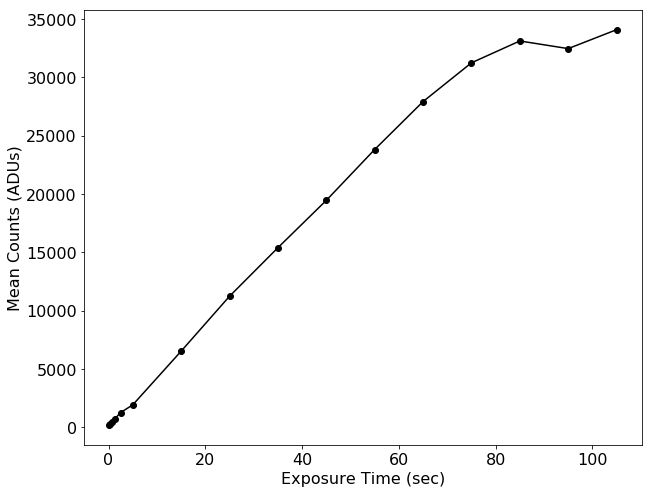
\includegraphics[width=0.8\linewidth]{linearity.png}
	\caption{A count against exposure time curve for the camera.}
	\label{fig:Linearity}
\end{figure}

\begin{table}[H]
	\centering
	\begin{tabular}{rl|rl}
		Exposure Time (s) & Mean Counts (ADUs) & Exposure Time (s) & Mean Counts (ADUs) \\ \hline
		0.16 & 185.59 & 35 & 15$\,$383.94 \rule{0pt}{14pt} \\
		0.312 & 260.67 & 45 & 19$\,$442.49 \rule{0pt}{14pt} \\
		0.625 & 402.87 & 55 & 23$\,$804.44 \rule{0pt}{14pt} \\
		1.25 & 698.58 & 65 & 27$\,$911.69 \rule{0pt}{14pt} \\
		2.5 & 1$\,$255.83 & 75 & 31$\,$235.74 \rule{0pt}{14pt} \\
		5 & 1$\,$912.06 & 85 & 33$\,$109.37 \rule{0pt}{14pt} \\
		15 & 6$\,$514.27 & 95 & 32$\,$454.10 \rule{0pt}{14pt} \\
		25 & 11$\,$222.69 & 105 & 34$\,$076.27 \rule{0pt}{14pt}
	\end{tabular}
	\caption{}
	\label{tab:Linearity}
\end{table}

It is important to note that changing the wavelength of the incident light does not change the linearity range or saturation type of a CCD, as those are purely a function of the full-well capacity, gain, and A/D converter capacity. These factors are not wavelength-dependent.

\subsection*{Dark Current and Band Gap Energy}

The band gap energy of a semiconductor -- such as the silicon of a CCD -- is how much energy it takes for an electron to go from the valence band to the conduction band. More simply, it's how much energy an electron needs to become mobile in the semiconductor. Thermal excitations may be enough to boost an electron to the conduction band, resulting in a false count in the CCD. The rate of these counts per pixel at 0$\,^{\circ}$C is the dark current of the CCD.

An empirical formula for the dark current of a CCD as a function of temperature is

\begin{equation}
D = 2.5\times10^{15} A I_d T^{1.5} e^\frac{E_g}{2 k T \rule{0pt}{5pt}}
\label{eq:DarkCurrent}
\end{equation}
where $T$ is temperature, $A$ is the pixel area, $I_d$ is the dark current at 300$\,$K, $k$ is Boltzmann's constant, and $E_g$ is the band gap energy of silicon.

Varying the temperature can damage the CCD, so we are using a set of data provided by the instructor. Both the data and a least squares fit of Equation \ref{eq:DarkCurrent} are graphed below.

\begin{figure}[H]
	\centering
	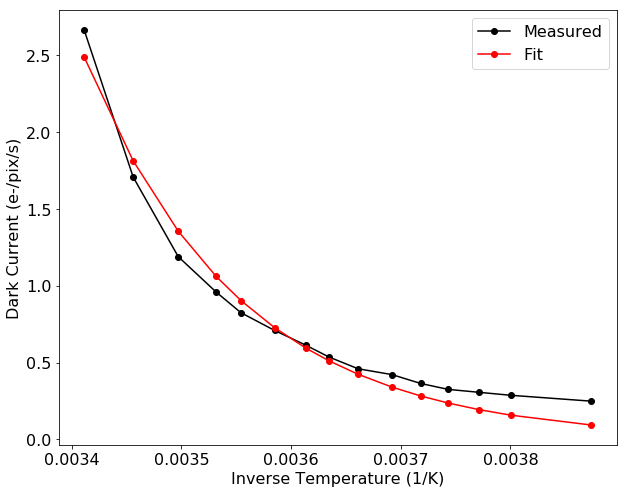
\includegraphics[width=0.8\linewidth]{DarkCurrent.png}
	\caption{The dark current as a function of CCD temperature for an SBIG ST-8XE camera.}
	\label{fig:DarkCurrent}
\end{figure}

From the same least-squares fit, we find a silicon band gap energy of 1.2$\,$eV. This differs by less than 10\% from the true value of 1.1$\,$eV.

Taking a closer look at Equation \ref{eq:DarkCurrent}, we see that it has a lower limit of 0 due to the $T^{1.5}$ term and exponential term approaching 0. The upper limit goes as $T^{1.5}$, as the exponential term approaches 1 for large $T$.

Finally, the measured dark current at 0$\,^{\circ}$C (0.00366$\,$1/K) is roughly 0.5$\,e^-$/pix/s. This is below the manufacturers stated 1$\,e^-$/pix/s, but of the same order. The difference may simply be chance, or it may be that the manufacturer releases conservative values to protect themselves from blame by customers. The latter seems more plausible.

\section*{Summary}

Our characterization of the CCD was a success. We were able to measure all important values to within 10\% of the manufacturer, and properly determined the saturation condition. The only major difference was in the dark current, though I suspect that is simply the manufacturer being conservative.

\end{document}